% !TeX program = pdflatex
\documentclass[11pt,a4paper]{article}

\usepackage[utf8]{inputenc}
\usepackage[T1]{fontenc}
\usepackage{times}
\usepackage[margin=1in]{geometry}
\usepackage{graphicx}
\usepackage{booktabs}
\usepackage{amsmath,amssymb}
\usepackage{multirow}
\usepackage{xcolor}
\usepackage{hyperref}
\usepackage{cleveref}
\usepackage{enumitem}
\usepackage{natbib}
\usepackage{microtype}
\usepackage[section]{placeins}
\usepackage{float}

\hypersetup{
    colorlinks=true,
    linkcolor=blue!70!black,
    citecolor=blue!70!black,
    urlcolor=blue!70!black,
    pdftitle={Do Multilingual VLMs Reason Equally? A Cross-Lingual Visual Reasoning Audit for Indian Languages},
    pdfauthor={Swastik R},
}

\newcommand{\pp}{\,\text{pp}}

\title{Do Multilingual VLMs Reason Equally?\\ A Cross-Lingual Visual Reasoning Audit\\ for Indian Languages}

\author{Swastik R\\[2pt]
\small Indian Institute of Information Technology, Raichur}

\date{}

\begin{document}
\maketitle

%% ===========================================================================
\begin{abstract}
Vision-language models score well on mathematical, scientific, and spatial reasoning benchmarks, yet these evaluations are overwhelmingly English.
I present the first cross-lingual visual reasoning audit for Indian languages.
980 questions from MathVista, ScienceQA, and MMMU are translated into Hindi, Tamil, Telugu, Bengali, Kannada, and Marathi using IndicTrans2, with Gemini 2.0 Flash cross-verification on 50 samples per language (inter-translator agreement 0.79--0.84).
Eight VLMs, from 7B open-source models to GPT-4o, are evaluated across all seven languages, yielding 68{,}600 inference records that include text-only and chain-of-thought ablations.
I find accuracy drops of 9.8--25 percentage points when switching from English to an Indian language, with Dravidian languages suffering up to 13.2$\pp$ more than Indo-Aryan.
Chain-of-thought prompting \emph{degrades} Bengali ($-$14.4$\pp$) and Kannada ($-$11.4$\pp$) rather than helping, exposing English-centric reasoning chains.
Aya-Vision-8B, built for 23 languages, still drops 28.5$\pp$ on Dravidian scripts; multilingual pretraining alone does not transfer visual reasoning.
I release the translated benchmark and all model outputs.\footnote{Code and data: \url{https://github.com/QuantumByte-01/multilingual-vlm-reasoning-audit}; HuggingFace: \url{https://huggingface.co/datasets/Swastikr/multilingual-vlm-reasoning}}
\end{abstract}

%% ===========================================================================
\section{Introduction}
\label{sec:intro}

India's 260 million school-age children study predominantly in regional-medium schools where the language of instruction is Hindi, Tamil, Telugu, Bengali, Kannada, or Marathi~\citep{nep2020}.
EdTech platforms are beginning to integrate vision-language models (VLMs) for automated tutoring and assessment, raising a practical question: can these models reason about mathematics and science \emph{in the student's own language}?

Existing benchmarks do not answer this.
Indian-language VLM evaluations probe cultural understanding~\citep{surana2026viraasat,maji2025drishtikon}, factual VQA~\citep{faraz2025indicvisionbench}, or broad multilingual proficiency~\citep{khan2025chitrarth}, but none isolate mathematical, scientific, or spatial reasoning.
India-focused VLM architectures such as Chitrarth~\citep{khan2025chitrarth} have been proposed, yet no benchmark exists to test whether they, or any other model, can actually solve Kannada science problems or Tamil geometry.

I address this gap by translating 980 visual reasoning questions from MathVista~\citep{lu2024mathvista}, ScienceQA~\citep{lu2022scienceqa}, and MMMU~\citep{yue2024mmmu} into six Indian languages with IndicTrans2~\citep{gala2023indictrans2}.
The images stay fixed across languages; only the question text changes.
Eight VLMs are evaluated (GPT-4o, Gemma~3-27B, Llama-4-Maverick, Qwen3-VL-30B, Qwen2.5-VL-32B, Qwen2.5-VL-7B, InternVL2.5-8B, and Aya-Vision-8B), together with text-only and chain-of-thought ablations on Qwen2.5-VL-7B, for a total of 68{,}600 inference records (\Cref{fig:heatmap}).

\begin{figure}[H]
\centering

\includegraphics[width=\textwidth]{fig1_heatmap.pdf}
\caption{Accuracy heatmap across eight models and seven languages. Every model degrades from English (left column) to Indian languages, with Dravidian languages (ta, te, kn) consistently darker than Indo-Aryan (hi, bn, mr).}
\label{fig:heatmap}
\end{figure}

My main findings:
\begin{itemize}[nosep,leftmargin=1.5em]
\item Gemma~3-27B shows the smallest average drop from English (9.8$\pp$); GPT-4o achieves the highest Indian-language accuracy (43.2\%); open-source models lose 15--25$\pp$.
\item Dravidian languages are harder than Indo-Aryan for every model, with the family gap reaching 13.2$\pp$ for Aya-Vision-8B.
\item Chain-of-thought prompting backfires in Indian languages: Bengali accuracy falls 14.4$\pp$ and Kannada 11.4$\pp$ relative to the standard prompt, indicating that the model's reasoning chains are locked to English.
\item Removing the image costs English 15.5$\pp$ but only 4.9--9.7$\pp$ for Indian languages, implying that models under-exploit visual information when text comprehension is weak.
\item Scaling from 7B to 32B within the Qwen2.5-VL family gains 4.3$\pp$ on Indian languages while losing 1.0$\pp$ on English; scale broadens linguistic coverage without improving reasoning.
\end{itemize}


%% ===========================================================================
\section{Related Work}
\label{sec:related}

\paragraph{Indian-language VLM benchmarks.}
IndicVisionBench~\citep{faraz2025indicvisionbench} covers 10 Indian languages with over 37K QA pairs but targets cultural understanding and OCR, not reasoning.
The BharatBench framework introduced in~\citet{khan2025chitrarth} spans speech, OCR, and embeddings without isolating STEM tasks.
VIRAASAT~\citep{surana2026viraasat} and DRISHTIKON~\citep{maji2025drishtikon} evaluate cultural knowledge and geographic diversity.
Chitrarth~\citep{khan2025chitrarth} introduces an India-focused VLM architecture but no reasoning-specific evaluation.
This work differs by holding the image fixed and varying only the question language, so that any accuracy change is directly attributable to language.

\paragraph{Multilingual VLM evaluation beyond India.}
MaRVL~\citep{liu2021marvl} tests visually grounded reasoning in five languages, including Tamil, but relies on culturally situated images and predates current VLMs.
xGQA~\citep{pfeiffer2022xgqa} extends GQA to seven languages, none Indian.
VLURes~\citep{atuhurra2025vlures} benchmarks four languages including Urdu.
ALM-Bench~\citep{vayani2024alm} and CVQA~\citep{romero2024cvqa} include partial Indian-language coverage but do not focus on reasoning.
Pangea~\citep{yue2024pangea}, a 39-language multimodal LLM, is the closest open-source multilingual effort, though it too lacks a reasoning-focused benchmark.

\paragraph{Visual reasoning benchmarks.}
MathVista~\citep{lu2024mathvista} evaluates mathematical reasoning in visual contexts; MATH-Vision~\citep{wang2024mathvision} extends this to competition-level problems.
ScienceQA~\citep{lu2022scienceqa} covers K-12 science with diagrams.
MMMU~\citep{yue2024mmmu} targets college-level STEM across 30 subjects.
All three are English-only; I extend them cross-lingually.

\paragraph{Multilingual reasoning in LLMs.}
\citet{shi2023mgsm} showed that English chain-of-thought outperforms native-language CoT on grade-school math in 10 languages, but without images.
\citet{ahuja2023mega} broadened multilingual generative evaluation across tasks and languages.
\citet{saji2025reasoning} study multilingual reasoning in language reasoning models on text-only benchmarks (MGSM, GPQA), finding that models default to English reasoning chains regardless of prompt language.
This paper extends this line of inquiry to the visual domain, where images may partly compensate for weak text comprehension.

\paragraph{Indian NLP resources.}
IndicTrans2~\citep{gala2023indictrans2} provides open-source neural machine translation for all 22 scheduled Indian languages and outperforms Google Translate and NLLB-54B.
I use it as the primary translation system, complemented by the broader Indic NLP infrastructure described by~\citet{doddapaneni2023towards}.


%% ===========================================================================
\section{Methodology}
\label{sec:method}

\subsection{Dataset Construction}

I assemble 980 visual reasoning questions from three sources:
\begin{itemize}[nosep,leftmargin=1.5em]
\item \textbf{MathVista}~\citep{lu2024mathvista}: 400 questions from the testmini split covering geometry, algebra, statistics, chart interpretation, and word problems.  Language-independent pattern-matching items (e.g., IQ-test sequences) were excluded.
\item \textbf{ScienceQA}~\citep{lu2022scienceqa}: 400 natural-science questions with images, spanning K-12 physics, chemistry, and biology.
\item \textbf{MMMU}~\citep{yue2024mmmu}: 180 STEM questions at the college level (mathematics, physics, engineering).
\end{itemize}
Each question is paired with an image that remains identical across languages; only the text changes.

\subsection{Languages}

I select six Indian languages spanning two major families and five scripts (\Cref{tab:languages}).
Hindi and Marathi share the Devanagari script but differ as languages, enabling us to separate vocabulary and training-data effects from script-level effects.
Tamil and Kannada share the Dravidian family but use distinct scripts, providing a complementary control.

\begin{table}[t]
\centering
\small
\caption{Target languages with script, family, and approximate L1 speaker population.}
\label{tab:languages}
\begin{tabular}{@{}llllr@{}}
\toprule
\textbf{Language} & \textbf{Code} & \textbf{Script} & \textbf{Family} & \textbf{L1 (M)} \\
\midrule
English & en & Latin & --- & --- \\
Hindi & hi & Devanagari & Indo-Aryan & 340 \\
Bengali & bn & Bengali & Indo-Aryan & 265 \\
Marathi & mr & Devanagari & Indo-Aryan & 83 \\
Tamil & ta & Tamil & Dravidian & 75 \\
Telugu & te & Telugu & Dravidian & 75 \\
Kannada & kn & Kannada & Dravidian & 44 \\
\bottomrule
\end{tabular}
\end{table}

\subsection{Translation}

All 980 questions are translated into each target language with IndicTrans2~\citep{gala2023indictrans2}.
Mathematical symbols ($\pi$, $\sqrt{\,}$, $=$), Arabic numerals, SI units, and answer labels (A/B/C/D) are preserved, consistent with conventions in Indian STEM education.
Technical terms are translated by IndicTrans2; instruction text is fully translated per language to test multilingual instruction following.

Translation quality is verified by independently translating 50 random samples per language with Gemini 2.0 Flash and computing inter-translator agreement (\Cref{tab:translation}).
Scores range from 0.79 (Kannada, Marathi) to 0.84 (Hindi), all above a 0.65 acceptance threshold.

\begin{table}[t]
\centering
\small
\caption{Inter-translator agreement between IndicTrans2 and Gemini 2.0 Flash on 50 random samples per language.}
\label{tab:translation}
\begin{tabular}{@{}lcccccc@{}}
\toprule
& hi & ta & bn & te & kn & mr \\
\midrule
Agreement & 0.844 & 0.811 & 0.806 & 0.803 & 0.791 & 0.791 \\
\bottomrule
\end{tabular}
\end{table}

\subsection{Models}

Eight VLMs are evaluated (\Cref{tab:models}).
Three open-source models (Qwen2.5-VL-7B, InternVL2.5-8B, Aya-Vision-8B) are served with vLLM on an AMD MI300X 192\,GB GPU in bfloat16.
Cloud models are accessed through Google AI (Gemma~3-27B), DeepInfra (Qwen2.5-VL-32B, Qwen3-VL-30B, Llama-4-Maverick in FP8), and OpenAI (GPT-4o).

Two ablations use Qwen2.5-VL-7B as a representative open-source model:
(i)~\textbf{No-image}, where the image is removed and only the question text is provided;
(ii)~\textbf{Chain-of-thought} (CoT), where ``Think step by step'' is appended to the prompt in the target language.

\begin{table}[t]
\centering
\small
\caption{Models evaluated. ``Overall'' is the macro-average accuracy across all seven languages.}
\label{tab:models}
\begin{tabular}{@{}llcr@{}}
\toprule
\textbf{Model} & \textbf{Access} & \textbf{Params} & \textbf{Overall (\%)} \\
\midrule
GPT-4o~\citep{openai2024gpt4o} & OpenAI API & --- & 44.8 \\
Qwen3-VL-30B~\citep{bai2025qwen3vl} & DeepInfra & 30B & 43.5 \\
Gemma~3-27B~\citep{google2025gemma3} & Google AI & 27B & 43.4 \\
Llama-4-Maverick~\citep{meta2025llama4} & DeepInfra & 17B$\times$128E & 42.6 \\
Qwen2.5-VL-32B~\citep{bai2025qwen25vl} & DeepInfra & 32B & 37.0 \\
Qwen2.5-VL-7B~\citep{bai2025qwen25vl} & MI300X (vLLM) & 7B & 33.5 \\
InternVL2.5-8B~\citep{chen2024internvl} & MI300X (vLLM) & 8B & 28.1 \\
Aya-Vision-8B~\citep{dash2025ayavision} & MI300X (vLLM) & 8B & 23.3 \\
\bottomrule
\end{tabular}
\end{table}

\subsection{Evaluation Protocol}

Each model receives the translated question, the original image, and a language-specific instruction asking for a letter answer (A--D) for MCQs or a number for free-form questions.
Temperature is set to 0 for reproducibility.

For multiple-choice questions (762 of 980), I extract the first standalone letter A--D from the response, also recognizing Devanagari and other script-specific option labels.
For free-form numerical questions (218 of 980), script-specific numerals (Devanagari, Bengali, Tamil, Telugu, Kannada) are converted to Arabic digits and a $\pm$5\% tolerance is applied.
Extraction failure rates are non-trivial for some models (33.9\% for Aya-Vision-8B, 25.0\% for InternVL2.5-8B); reported accuracies for these models should be interpreted as lower bounds.

All accuracies are accompanied by 95\% bootstrap confidence intervals ($N{=}2{,}000$ resamples).
Pairwise comparisons between English and each Indian language use McNemar's test; all are significant at $p < 0.001$.


%% ===========================================================================
\section{Results}
\label{sec:results}

\subsection{Overall Accuracy}

\Cref{tab:main} presents the full results.
GPT-4o achieves the highest average accuracy on Indian languages (43.2\%), while Gemma~3-27B, despite lower English accuracy, drops only 9.8$\pp$---the best language robustness among all models tested.
At the other extreme, Qwen3-VL-30B posts the highest English accuracy (64.9\%) but loses 24.9$\pp$ when switching to Indian languages, indicating that strong English performance does not automatically generalize cross-lingually.

Among the 7--8B open-source models, accuracy drops range from 20.4$\pp$ (InternVL2.5-8B) to 21.9$\pp$ (Aya-Vision-8B).
Refusal rates remain below 3\% across all models and languages, so the accuracy losses reflect genuine reasoning failures rather than model refusals.

\begin{table*}[t]
\centering
\small
\caption{Accuracy (\%) per model and language.  95\% bootstrap CIs are shown for the English column; all non-English comparisons are significant at $p<0.001$ (McNemar's test).  ``Drop'' is the difference between English accuracy and the mean accuracy across the six Indian languages.}
\label{tab:main}
\begin{tabular}{@{}l r@{\,}l ccccccc@{}}
\toprule
\textbf{Model} & \multicolumn{2}{c}{\textbf{en}} & \textbf{hi} & \textbf{ta} & \textbf{te} & \textbf{bn} & \textbf{kn} & \textbf{mr} & \textbf{Drop} \\
\midrule
Qwen3-VL-30B        & \textbf{64.9} & {\scriptsize[61.9--68.0]}  & 44.1 & 41.1 & 36.5 & 43.3 & 38.7 & 36.1 & 24.9\,$\pp$ \\
Llama-4-Maverick     & 55.4 & {\scriptsize[52.2--58.6]}  & 43.4 & 34.9 & 38.6 & 42.7 & 41.6 & 41.9 & 14.9\,$\pp$ \\
GPT-4o               & 54.5 & {\scriptsize[51.4--57.6]}  & \textbf{44.6} & \textbf{40.5} & \textbf{43.0} & \textbf{44.5} & \textbf{43.7} & \textbf{43.2} & \textbf{11.3}\,$\pp$ \\
Gemma~3-27B          & 51.8 & {\scriptsize[48.9--55.0]}  & 42.0 & 41.9 & 42.5 & 41.9 & 41.3 & 42.2 & 9.8\,$\pp$ \\
Qwen2.5-VL-7B       & 51.3 & {\scriptsize[48.2--54.4]}  & 34.2 & 28.7 & 26.9 & 32.7 & 30.6 & 30.0 & 20.8\,$\pp$ \\
Qwen2.5-VL-32B      & 50.3 & {\scriptsize[47.1--53.5]}  & 34.1 & 34.2 & 33.2 & 39.1 & 32.5 & 35.6 & 15.5\,$\pp$ \\
InternVL2.5-8B       & 45.6 & {\scriptsize[42.5--48.9]}  & 29.8 & 22.4 & 22.9 & 24.9 & 23.6 & 27.9 & 20.4\,$\pp$ \\
Aya-Vision-8B        & 42.0 & {\scriptsize[38.8--45.0]}  & 33.6 & 14.9 & 11.6 & 21.7 & 14.2 & 25.1 & 21.9\,$\pp$ \\
\midrule
\multicolumn{10}{@{}l}{\textit{Ablations (Qwen2.5-VL-7B)}} \\
No-image             & 35.8 &  & 26.0 & 19.0 & 20.7 & 24.5 & 23.7 & 25.1 & 12.7\,$\pp$ \\
Chain-of-thought     & 49.5 &  & 25.0 & 29.7 & 22.8 & 18.3 & 19.2 & 33.3 & 24.8\,$\pp$ \\
\bottomrule
\end{tabular}
\end{table*}


\subsection{Language Family Effect}

\Cref{tab:family} and \Cref{fig:drop} disaggregate the accuracy drop by language family and language respectively.
Dravidian languages (Tamil, Telugu, Kannada) consistently lose more accuracy than Indo-Aryan (Hindi, Bengali, Marathi).
The gap is modest for GPT-4o (1.7$\pp$) and essentially absent for Gemma~3-27B (0.1$\pp$), but reaches 13.2$\pp$ for Aya-Vision-8B, a model whose pretraining explicitly covers several Indian languages.
A model trained on Indian languages can still exhibit a 13$\pp$ family gap, suggesting that the bottleneck lies in reasoning transfer rather than surface-level language coverage.

\begin{table}[t]
\centering
\small
\caption{Accuracy drop from English ($\pp$), averaged within each language family.  ``Gap'' is Dravidian drop minus Indo-Aryan drop.}
\label{tab:family}
\begin{tabular}{@{}lccc@{}}
\toprule
\textbf{Model} & \textbf{Indo-Aryan} & \textbf{Dravidian} & \textbf{Gap} \\
\midrule
Aya-Vision-8B     & 15.2 & 28.5 & \textbf{+13.2} \\
InternVL2.5-8B    & 18.1 & 22.7 & +4.6 \\
Llama-4-Maverick  & 12.8 & 17.0 & +4.3 \\
Qwen2.5-VL-7B    & 19.1 & 22.6 & +3.5 \\
Qwen2.5-VL-32B   & 14.1 & 17.0 & +3.0 \\
Qwen3-VL-30B     & 23.7 & 26.1 & +2.4 \\
GPT-4o            & 10.4 & 12.1 & +1.7 \\
Gemma~3-27B       & 9.8  & 9.9  & ${\sim}$0 \\
\bottomrule
\end{tabular}
\end{table}

\begin{figure}[H]
\centering

\includegraphics[width=\columnwidth]{fig2_accuracy_drop.pdf}
\caption{Average accuracy drop from English, per language, averaged across models.  Dravidian languages (ta, te, kn) consistently suffer larger drops than Indo-Aryan (hi, bn, mr).}
\label{fig:drop}
\end{figure}

\paragraph{Script versus language.}
Hindi and Marathi both use Devanagari, yet Marathi drops an average of 3.0$\pp$ more than Hindi across models.
The gap persists even for Aya-Vision-8B, where Marathi accuracy is 8.5$\pp$ lower than Hindi despite sharing the same script.
Training data volume, rather than script encoding, appears to be the dominant factor.


\subsection{Per-Dataset Patterns}

\Cref{tab:per_dataset} and \Cref{fig:per_dataset} break accuracy drops down by source dataset.
Two patterns stand out.
First, MathVista produces the largest drops for high-performing models (Qwen3-VL-30B loses 29.3$\pp$), consistent with math word problems requiring precise language comprehension.
Second, Gemma~3-27B shows a \emph{negative} ScienceQA drop ($-$2.7$\pp$): its Indian-language accuracy slightly exceeds English.
A plausible explanation is that ScienceQA's biology and physics diagrams carry enough visual signal for the correct answer regardless of question language, and Gemma's post-training alignment is particularly effective at exploiting this.

At the other end, Aya-Vision-8B and InternVL2.5-8B lose 36--38$\pp$ on ScienceQA, pointing to heavy reliance on English science vocabulary.

\begin{table}[t]
\centering
\small
\caption{Accuracy drop ($\pp$) from English to average Indian-language accuracy, by source dataset.}
\label{tab:per_dataset}
\begin{tabular}{@{}lccc@{}}
\toprule
\textbf{Model} & \textbf{MathVista} & \textbf{ScienceQA} & \textbf{MMMU} \\
\midrule
GPT-4o            & 17.2 & 7.0   & 7.3 \\
Gemma~3-27B       & 24.3 & $-$2.7 & 5.4 \\
Llama-4-Maverick  & 15.2 & 15.7  & 12.3 \\
Qwen3-VL-30B     & 29.3 & 21.5  & 22.8 \\
Qwen2.5-VL-32B   & 10.2 & 23.2  & 10.3 \\
Qwen2.5-VL-7B    & 20.5 & 24.8  & 12.9 \\
InternVL2.5-8B    & 8.1  & 36.8  & 11.4 \\
Aya-Vision-8B     & 9.3  & 38.4  & 13.1 \\
\bottomrule
\end{tabular}
\end{table}

\begin{figure}[H]
\centering

\includegraphics[width=\textwidth]{fig4_per_dataset.pdf}
\caption{Per-dataset accuracy for English versus the average across Indian languages.  MathVista shows the largest drops for most models.  Gemma~3-27B achieves a negative drop on ScienceQA (Indian languages outperform English).}
\label{fig:per_dataset}
\end{figure}

\Cref{fig:radar} complements the above by showing per-language accuracy across all three datasets simultaneously.
Hindi and Bengali consistently outperform Dravidian languages on MathVista and MMMU, while the gap narrows on ScienceQA where diagram-level visual signals partially compensate for weaker language understanding.

\begin{figure}[H]
\centering
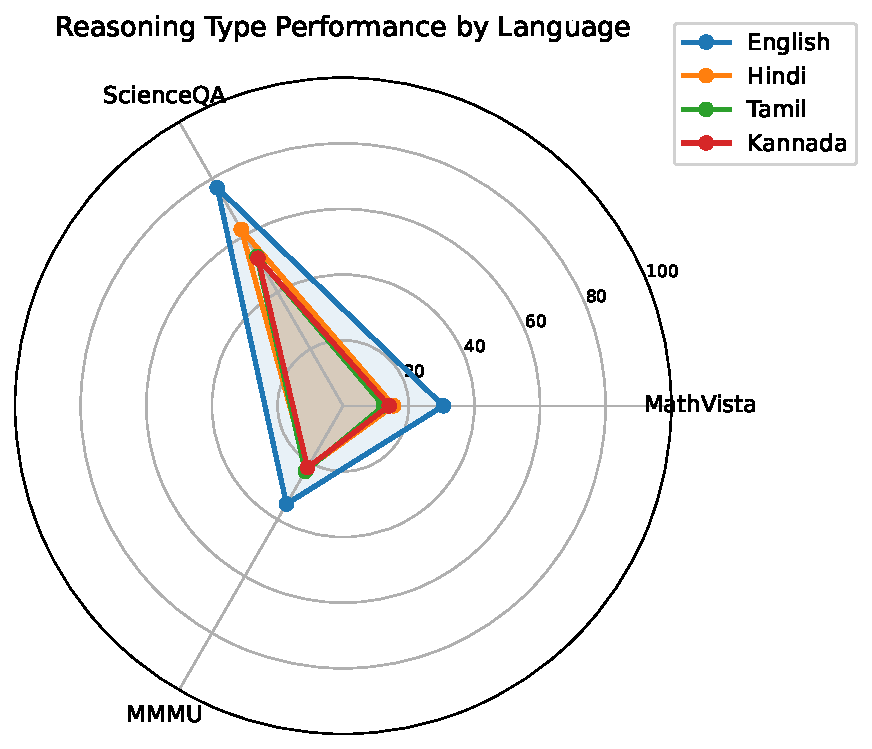
\includegraphics[width=\columnwidth]{fig3_radar.pdf}
\caption{Radar chart of accuracy per source dataset for each language (averaged over all models). English sets the outer reference; Dravidian languages (Tamil, Telugu, Kannada) cluster closer to the centre on MathVista and MMMU, confirming that reasoning-heavy tasks suffer the most.}
\label{fig:radar}
\end{figure}

\subsection{Cross-Lingual Consistency}

For each question, I check whether the model produces the same extracted answer across all languages for which a valid answer was obtained (restricting to questions with at least four successful extractions out of seven).
Observed agreement rates range from 67.1\% (Aya-Vision-8B) to 80.8\% (Llama-4-Maverick), well above the near-zero level expected from independent random guessing on four-choice MCQs (\Cref{fig:consistency}).
All models engage in non-trivial cross-lingual reasoning, but the least consistent models are the same ones with the highest accuracy drops, suggesting that language-dependent instability and accuracy loss share a common cause.

\begin{figure}[H]
\centering

\includegraphics[width=\columnwidth]{fig6_consistency.pdf}
\caption{Cross-lingual consistency: percentage of questions receiving the same extracted answer across all languages with valid extractions ($\geq$4 of 7).}
\label{fig:consistency}
\end{figure}


\subsection{Ablation: Image Removal and Chain-of-Thought}
\label{sec:ablation}
\Cref{fig:ablation} shows per-language accuracy for the three Qwen2.5-VL-7B variants.

\begin{figure}[H]
\centering

\includegraphics[width=\columnwidth]{fig7_ablation.pdf}
\caption{Ablation results for Qwen2.5-VL-7B.  Removing the image hurts all languages; chain-of-thought hurts most Indian languages while leaving English roughly unchanged.}
\label{fig:ablation}
\end{figure}

\paragraph{Image removal.}
Stripping the image from the prompt reduces English accuracy by 15.5$\pp$ (from 51.3\% to 35.8\%).
Indian-language accuracy drops less, between 4.9$\pp$ (Marathi) and 9.7$\pp$ (Tamil).
The asymmetry is informative: models extract more from the image when they understand the text well; when text comprehension is weaker (as in Indian languages), the image is already under-utilized, so removing it costs less.

\paragraph{Chain-of-thought.}
Appending ``Think step by step'' barely changes English accuracy ($-$1.8$\pp$) but severely degrades Bengali ($-$14.4$\pp$), Kannada ($-$11.4$\pp$), and Hindi ($-$9.2$\pp$).
An interesting exception is Marathi, where CoT actually \emph{improves} accuracy by 3.3$\pp$, possibly reflecting stronger Devanagari-script training data for reasoning tasks.
In general, the model cannot sustain coherent step-by-step reasoning in languages where it lacks fluency; forcing it to do so produces garbled intermediate steps that corrupt the final answer.
This mirrors the text-only finding of \citet{shi2023mgsm} that English CoT outperforms native-language CoT, and extends it to visual reasoning.


\subsection{Effect of Scale}

Comparing Qwen2.5-VL-7B with Qwen2.5-VL-32B (same architecture family) shows that the larger model gains 4.3$\pp$ on Indian languages while losing 1.0$\pp$ on English.
The English-to-Indian-language drop shrinks from 20.8$\pp$ (7B) to 15.5$\pp$ (32B): a meaningful reduction, but far from closing the gap.
Scale appears to broaden linguistic coverage without fundamentally improving cross-lingual reasoning transfer.


%% ===========================================================================
\section{Analysis}
\label{sec:analysis}

\Cref{fig:family} plots each model's Indo-Aryan drop against its Dravidian drop; all points lie above the diagonal, confirming that Dravidian languages are consistently harder.

\begin{figure}[H]
\centering
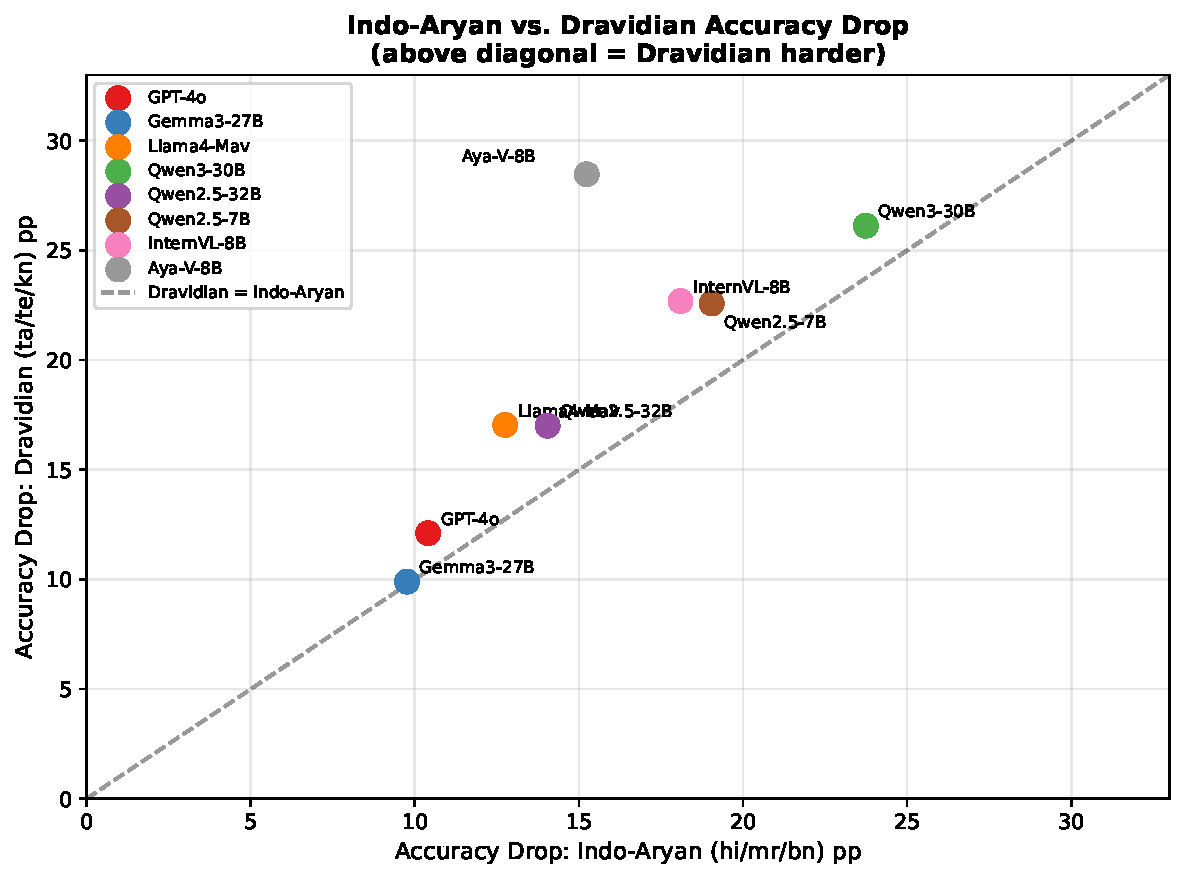
\includegraphics[width=\columnwidth]{fig8_family_scatter.pdf}
\caption{Accuracy drop ($\pp$) from English, Indo-Aryan vs.\ Dravidian.  Points above the diagonal mean Dravidian languages are harder.  Gemma~3-27B is the only model near the diagonal.}
\label{fig:family}
\end{figure}


\subsection{English Token Leak}

To probe for covert English reasoning, I measure the fraction of ${\geq}3$-letter English words in non-English responses (\Cref{fig:leak}).
Llama-4-Maverick stands out with 32\% English tokens on average across Indian-language responses.
It evidently reasons in English and switches to the target script only superficially, yet it achieves the highest cross-lingual consistency (80.8\%), meaning its English-leaked reasoning is often \emph{correct}.

At the opposite end, Aya-Vision-8B produces only 0.8\% English tokens but has the lowest consistency (67.1\%).
Faithfully generating in the target script does not entail correct reasoning.

\begin{figure}[H]
\centering

\includegraphics[width=\columnwidth]{fig9_english_leak.pdf}
\caption{English token leak in non-English responses (percentage of ${\geq}$3-letter English words).  Llama-4-Maverick code-switches heavily at 32\%.}
\label{fig:leak}
\end{figure}


\subsection{Language Confusion}

I flag responses longer than 15 characters that contain no characters from the expected Unicode script range (\Cref{fig:confusion}).
Qwen3-VL-30B (1.2\% confusion) and Aya-Vision-8B (2.5\%) consistently respond in the target script.
GPT-4o registers 45\% apparent confusion, but this is largely an artifact of its terse single-letter MCQ answers (e.g., ``B''), which contain no script-specific characters by construction.

\begin{figure}[H]
\centering

\includegraphics[width=\columnwidth]{fig5_confusion_heatmap.pdf}
\caption{Language confusion rate: percentage of verbose ($>$15~character) responses containing no characters from the expected Unicode script range.}
\label{fig:confusion}
\end{figure}


\subsection{Response-Length Patterns}

Response length reveals strategy differences across models (\Cref{fig:length}).
Llama-4-Maverick generates uniformly verbose output (${\sim}$840--1{,}070 characters) regardless of language; it always writes out full reasoning.
Aya-Vision-8B produces \emph{longer} responses in Indian languages (310--514 characters) than in English (123 characters), possibly reflecting lower confidence and compensatory over-generation.
InternVL2.5-8B shows the reverse: 6-character English responses (single-letter MCQ answers) but full-sentence Indian-language output, which partly explains its elevated confusion rate.

\begin{figure}[H]
\centering

\includegraphics[width=\columnwidth]{fig10_response_length.pdf}
\caption{Response length ratio relative to English.  Values above 1 indicate longer responses in the target language.}
\label{fig:length}
\end{figure}


\subsection{MCQ versus Free-Form Questions}

Free-form numerical questions suffer disproportionately.
Qwen2.5-VL-32B reaches 63.9\% on MCQs but only 2.8\% on free-form numerical questions in English: it generates extended reasoning without a clean final number, causing extraction failures.
This 61$\pp$ MCQ--free-form gap is the largest in the set and highlights that reported accuracy is heavily influenced by answer extraction quality.
InternVL2.5-8B shows a similar pattern (52.5\% MCQ vs.\ 21.6\% free-form).


%% ===========================================================================
\section{Discussion}
\label{sec:discussion}

\paragraph{Educational implications.}
India's National Education Policy 2020~\citep{nep2020} mandates mother-tongue instruction through Grade~5.
If the best available VLM drops 11.3$\pp$ on STEM reasoning when asked in an Indian language, and open-source alternatives drop 15--25$\pp$, deploying these models as tutoring tools in regional-medium schools risks systematically disadvantaging non-English students.
The problem is most acute in Dravidian-medium schools, where drops reach 12--28$\pp$ depending on model.

\paragraph{Multilingual pretraining is not enough.}
Aya-Vision-8B is trained on 23 languages, several of them Indian.
It faithfully responds in target scripts (0.8\% English leak) and rarely refuses.
Yet it drops 28.5$\pp$ on Dravidian languages and has the lowest cross-lingual consistency.
The model can produce Tamil text; it cannot reason in Tamil.
Closing this gap likely requires multilingual \emph{reasoning} fine-tuning on STEM-specific data, not simply broader pretraining corpora.

\paragraph{Gemma~3-27B as an outlier.}
Gemma~3-27B is the only model with a near-zero Dravidian--Indo-Aryan gap (0.1$\pp$) and actually gains accuracy on ScienceQA when switching from English.
While the full training recipe is not public, this suggests that targeted multilingual alignment during post-training can effectively equalize performance across language families, a concrete design goal for future models.

\paragraph{Chain-of-thought: handle with care.}
Chain-of-thought prompting is widely assumed to be beneficial for reasoning tasks.
The results show it is counterproductive in Indian languages, with the exception of Marathi.
The reasoning chain becomes a bottleneck when the model lacks the fluency to sustain coherent logic in the target language.
Practitioners deploying VLMs in multilingual settings should avoid CoT prompting unless the model has been specifically tuned for non-English reasoning chains.

\paragraph{The hidden-English pattern.}
Llama-4-Maverick's combination of 32\% English token leak and 80.8\% cross-lingual consistency points to a strategy where the model reasons internally in English and translates at the surface.
This yields correct MCQ answers but would likely break down for generative tasks such as tutoring, explanation, and feedback, which require fluent target-language output.


%% ===========================================================================
\section{Limitations}
\label{sec:limits}

The translations rely on IndicTrans2 with Gemini 2.0 Flash cross-verification (agreement 0.79--0.84).
Machine translation errors, particularly for technical terms, may introduce noise; native-speaker validation on a larger sample would strengthen the benchmark.
Only 6 of India's 22 scheduled languages are covered; low-resource languages like Odia and Assamese, and the over 100 non-scheduled languages, remain untested.
The source benchmarks were designed for English speakers and may carry cultural or curricular biases that affect all translations equally.
High extraction failure rates for Aya-Vision-8B (33.9\%) and InternVL2.5-8B (25.0\%) mean that these models' true reasoning capability may be higher than the reported numbers.
API-based models may be updated over time; the results reflect a snapshot taken in March~2026.


%% ===========================================================================
\section{Conclusion}
\label{sec:conclusion}

This audit---980 questions, seven languages, eight models, 68{,}600 inference records---documents a systematic 9.8--25$\pp$ accuracy penalty when VLMs reason in Indian languages instead of English.
Dravidian languages are consistently harder than Indo-Aryan.
Chain-of-thought prompting backfires in most Indian languages; multilingual pretraining alone does not transfer reasoning; and scale narrows but does not close the gap.
These findings argue for mandatory multilingual reasoning evaluation before VLMs are deployed in Indian educational settings.

The translated benchmark, model outputs, and evaluation code are publicly available at \url{https://github.com/QuantumByte-01/multilingual-vlm-reasoning-audit} and on HuggingFace.\footnote{\url{https://huggingface.co/datasets/Swastikr/multilingual-vlm-reasoning}}


%% ===========================================================================
\section*{Acknowledgments}

Open-source model inference was conducted on an AMD Instinct MI300X GPU with 192\,GB HBM3 memory.
Cloud inference used the Google AI, DeepInfra, and OpenAI APIs.

\bibliographystyle{plainnat}
\bibliography{references}

\end{document}
